\lab{Git}{Git}
\label{appendix:git}
\objective{
Computer code is delicate.
A rogue or clumsy programmer can easily damage a program with a simple spelling error.
Maintaining a working product is therefore a serious endeavor in software development, requiring checks, collaboration, and careful coordination.
\emph{Git} is a version control system that facilitates code development involving multiple contributors.
It is commonly used to manage large projects, especially open-source projects, but it can also be used for personal code storage and management.
In this appendix we introduce Git and Bitbucket, a web-based hosting service for Git.
This tutorial does not require any previous programming experience.
}

% This appendix is meant to be general and not provide classroom-specific instructions. See byuacmegit.tex in this folder ACME-specific instructions.

\section*{Overview} % =========================================================

The main idea behind Git is that the master copy (the official version) of a program's code is kept in the cloud in a \emph{repository}.
All certified contributors can \emph{clone} the repository onto their machine so that they can make changes to the code.
All changes are then submitted to the cloud, reviewed, and approved before the changes are \emph{merged} into the master copy.

If two contributors make changes to the same piece of code, it may create a \emph{merge conflict}, which must be resolved before any changes can be merged in.
For small repositories with few collaborators, merge conflicts are very rarely a problem.
The main issue then becomes understanding how to communicate edits between a local copy and the master copy in the cloud.

\subsection*{Installation} % --------------------------------------------------

Download the appropriate installer at \url{http://git-scm.com/downloads}.
Git is underlying software that will be accessed through the command line, so the installation will not create a new visible application.
On Windows machines, however, it will also download a terminal-like interface just for Git called \emph{git bash}.
Most Linux and Macintosh machines come with Git pre-installed.

\subsection*{Creating a New Repository} % -------------------------------------

A repository is the place where all of the code for an associated project resides.
Many different companies have websites for hosting Git repositories, including
\href{https://github.com/}{Github}, \href{https://bitbucket.org/}{Bitbucket}, \href{https://gitlab.com/}{Gitlab}, and others.
Github is by far the most popular, especially for open-source projects, but Bitbucket offers free private repositories.

There are two ways to set up a new repository: by importing an existing repository, or by starting from scratch.
Imported repositories are ready to be cloned, but new or empty repositories require a little more setup.

Once a new or empty repository has been created on-line, it must be manually connected to a local folder on a computer.
On your machine, navigate  to the location where you would like the repository to reside locally via the terminal (on Windows, use the Git bash application).
Then execute the following bash commands:

\begin{lstlisting}[language=bash]
$ mkdir /path/to/your/project       # Make a new directory for the repository.
$ cd /path/to/your/project          # Enter the new directory.
$ git init                          # Turn the directory into a Git folder.
# Finally, connect the local folder to the repository in the cloud.
$ git remote add origin https://<host website>/<username>/<repo_name>
\end{lstlisting}
The key word ``origin'' now references the repository in the cloud.

\subsection*{Cloning a Repository} % ------------------------------------------

Existing or imported repositories may be \emph{cloned} into a local folder.
On your machine, navigate to the location where you would like to place the repository.
Execute the command \li{git clone <repo_url> <directory_name>}, where \li{<repo\_url>} is the web address to the repository and \li{<directory_name>} is the name of the new local directory for the repository.
This command creates a folder, places all files from the repository in that folder, and automatically connects the folder to the on-line repository via the alias ``origin.''
You may be asked to enter in your credentials to authenticate the cloning process.

\section*{Using Git} % ========================================================

Git has various commands for managing edits to a repository.
Execute \li{<<git help>>} in the command line for general help, or run \li{<<git help <command>>>} for instructions on a specific command.

The four most used git commands are as follows:
\begin{itemize}
\item \li{git pull origin master}: Pull updates from the on-line repository and synchronize with the local folder.
\item \li{git add <filename>}: Add a file to be tracked by the repository. Untracked files may remain in the local folder but will not be stored in the on-line repository.
\item \li{<<git commit -m "<descrption>">>}: Create a checkpoint in the repository history with a description of the changes.
\item \li{git push origin master}: Push committed changes up to the on-line repository.
\end{itemize}
A typical work session using git might look like the following:

\begin{lstlisting}[language=bash]
$ cd myRepo

# Update the local repository.
$ git pull origin master

# Make changes to the local repo.
# For example, create and save a file called 'text.txt'
$ touch text.txt

# Add new or changed files and commit the changes.
$ git add text.txt
$ git commit -m "Added test.txt to the repository."

# Push the changes to the on-line repository.
$ git push origin master
\end{lstlisting}

Commit often and with informative messages so you track your progress.

\begin{figure}[H]
\centering
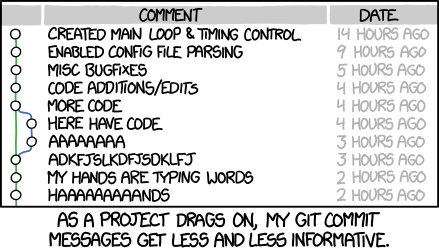
\includegraphics[width=.7\textwidth]{xkcd2.png}
\caption{\url{https://xkcd.com/1296/}}
\end{figure}

\subsection*{Branches} % ------------------------------------------------------

A \emph{branch} is a separate version of the repository.
The default branch is usually called \li{master}.
Use branches to keep track of edits on different projects.

\subsection*{Pull Requests} % -------------------------------------------------

TODO

\subsection*{Special Files} % -------------------------------------------------

\begin{itemize}
\item \texttt{.gitignore}: Specifies files to ignore in the index.
\item \texttt{.gitmodules}: Details connections to other repositories.
\item \texttt{.gitconfig}: Stores user name and like information.
\item \texttt{README.md}: A quick summary that will be rendered and displayed on-line at the repository host site.
\end{itemize}

\subsection*{Index of Git Commands} % -----------------------------------------

\begin{table}[H]
\centering
\begin{tabular}{l|l}
Command & Description \\ \hline
\li{git pull origin master} & Pull down changes from the master copy (synchronize).\\
\li{git add <filename(s)>} & Add a file or files to the list of things to be synced.\\
\li{git commit -m <<\"<message>\">>} & Package up the changes and give them a label (checkpoint).\\
\li{git push origin master} & Push committed changes up to the master copy\\
\li{git status} & See which files have been changed and which have been\\&added to the commit.\\
\li{git diff <filename>} & See the changes made on a particular file since the\\&latest commit.\\
\li{git checkout -- <filename>} & Revoke the changes made since the last commit.\\
\li{git log} & See the commit history.\\
\li{git revert} & Revert to the state of the last commit.
\end{tabular}
\end{table}

\begin{figure}
\centering

\includegraphics[width=\textwidth]{xkcd1.png}
\caption{\url{https://xkcd.com/1597/}}
\end{figure}

